\documentclass[11pt]{beamer}
\usepackage[utf8]{inputenc}
\usepackage[spanish]{babel}
\usepackage{amsmath,amsfonts,amssymb}
\usepackage{graphicx,booktabs,multirow,xcolor,colortbl}
\usepackage{hyperref,url,multicol,float}

\usetheme{Madrid}
\definecolor{mycyan}{RGB}{0,89,97}
\setbeamercolor{structure}{fg=mycyan}
\setbeamercolor{block title}{fg=white, bg=mycyan}
\setbeamercolor{block body}{bg=mycyan!10}
\setbeamercolor{alerted text}{fg=mycyan}

\author[Mecánica estadística]{Juan David Chaparro Rojas\\
Miguel Ángel Ramos Higuera\\
Samuel Homez Caicedo
}
\title{Modelo de Ising para Criminalidad en Bogotá}
\subtitle{Proyecto final mecánica estadística 2026-1}
\date{11 de junio de 2026}
\logo{
\includegraphics[scale=0.07]{sm.png}}
\institute[UD]{Programa académico de Física\\
Facultad de ciencias matemáticas y naturales\\
Universidad Distrital Francisco José de Caldas}

\AtBeginSection[]{\begin{frame}{Contenido}\tableofcontents[currentsection]\end{frame}}

\begin{document}

\begin{frame}
		\maketitle
	\end{frame}


\begin{frame}{Contenido}\tableofcontents\end{frame}

% ==================== SECCIÓN 1 ====================
\section{Introducción y Marco Teórico}

\begin{frame}{Motivación y Objetivos}

\textbf{Problema:} Bogotá presenta patrones criminales complejos en espacio y tiempo. Los enfoques tradicionales no incorporan simultáneamente la \textbf{dinámica temporal} ni la \textbf{interacción espacial}.

\vspace{0.3cm}
\textbf{Solución:} La física estadística ofrece el \textbf{modelo de Ising} (Lenz, 1920) para modelar sistemas de partículas interactuantes. Adaptándolo, cada UPZ es un ``espín'' que interactúa con sus vecinas.

\vspace{0.3cm}
\textbf{Objetivos:}
\begin{enumerate}[label=\alph*)]
    \item Adaptar el modelo de Ising a la dinámica criminal en Bogotá.
    \item Estimar el contagio $J$ y los campos locales $h_i$ con datos reales.
    \item Explicar $h_i$ mediante variables socioeconómicas observables.
    \item Validar la capacidad predictiva del modelo.
    \item Derivar implicaciones para política pública.
\end{enumerate}
\end{frame}

\begin{frame}{Fundamentos del Modelo de Ising}

\textbf{Hamiltoniano:} $\displaystyle H = -J \sum_{\langle i,j \rangle} s_i s_j - \sum_i h_i s_i$

\vspace{0.2cm}
\textbf{Distribución de Boltzmann:} $\displaystyle P(\{s\}) = \frac{1}{Z} \exp\!\left(-\frac{H}{k_B T}\right)$

\vspace{0.3cm}
\textbf{Observables macroscópicos:}
\[
M = \frac{1}{N}\sum s_i \qquad
C = \frac{1}{E}\sum_{\langle i,j \rangle} s_i s_j \qquad
\chi = N \cdot \text{Var}(M)
\]

\vspace{0.3cm}
\begin{table}[h]
\centering
\small
\begin{tabular}{l l l}
\toprule
\textbf{Física} & \textbf{Símbolo} & \textbf{Criminología} \\
\midrule
Espín & $s_i = \pm 1$ & UPZ con alta/baja actividad \\
Interacción & $J$ & Contagio criminal entre vecinos \\
Campo externo & $h_i$ & Vulnerabilidad intrínseca UPZ \\
Temperatura & $T$ & Impredictibilidad del sistema \\
\bottomrule
\end{tabular}
\end{table}
\end{frame}

\begin{frame}{Modelo Dinámico y Sociofísico}

\textbf{Predicción temporal (Markoviana):}
\[
P(s_i(t+1)=+1 \mid \mathbf{s}(t)) = \sigma\!\left(J \sum_{j \in \partial i} s_j(t) + h_i\right)
\]
$\sigma(x) = 1/(1+e^{-x})$: función sigmoide. $\partial i$: vecinos de la UPZ $i$.

\vspace{0.3cm}
\textbf{Modelo enriquecido con covariables $\mathbf{X}_i$:}
\[
P(s_i=+1) = \sigma\!\left(J_i(\mathbf{X}) \sum_{j \in \partial i} s_j + h_i(\mathbf{X})\right)
\]
\[
J_i = \beta_0 + \sum \beta_k X_{ik} \qquad
h_i = \alpha_0 + \sum \alpha_k X_{ik}
\]

\vspace{0.2cm}
$\beta_k > 0$: $X_k$ amplifica contagio. $\beta_k < 0$: bloquea.\\
$\alpha_k > 0$: $X_k$ aumenta crimen local. $\alpha_k < 0$: reduce.
\end{frame}

% ==================== SECCIÓN 2 ====================
\section{Datos y Metodología}

\begin{frame}{Fuentes de Datos y Construcción del Sistema}

\begin{table}[h]
\centering
\small
\begin{tabular}{l l l}
\toprule
\textbf{Fuente} & \textbf{Registros} & \textbf{Período} \\
\midrule
Llamadas Línea 123 & 1,068,340 & 2015--2026 \\
Estratificación (Manzanas) & 39,150 & 2025 \\
Deserción Escolar (UPZ) & 118 & 2024 \\
CAIs (Policía Nacional) & 154 & 2024 \\
Shapefile UPZ (SDP) & 113 & 2023 \\
\bottomrule
\end{tabular}
\end{table}

\vspace{0.2cm}
\textbf{Definición de espines} (percentiles históricos por UPZ):
\[
s_i(t) = \begin{cases}
+1 & \text{si incidentes} > P_{70}^{(i)} \\
-1 & \text{si incidentes} < P_{30}^{(i)} \\
0  & \text{otro caso}
\end{cases}
\]

Matriz: 135 meses $\times$ 124 UPZs. Red: 111 nodos, 302 aristas.\\
$M_{\text{obs}}=-0.067$, $C_{\text{obs}}=0.121$ ($p<0.001$), $\chi_{\text{obs}}=2.78$.
\end{frame}

\begin{frame}{Pipeline de Procesamiento}

\begin{enumerate}
    \item \textbf{Carga:} 1.07M registros CSV. Filtrado: 7 delitos de alto impacto.
    \item \textbf{Espines:} Agrupación UPZ-mes, pivoteo, percentiles, binarización.
    \item \textbf{Red:} Shapefile $\to$ adyacencias $\to$ matriz $A_{ij}$ (302 aristas).
    \item \textbf{Datos dinámicos:} Pares $(t, t+1)$ con estado objetivo y suma de vecinos.
    \item \textbf{Modelo base:} Regresión logística L2 $\to$ $J=0.4336$, 111 valores $h_i$.
    \item \textbf{Datos abiertos:} Carga de SHP externos, asignación espacial, 7 covariables.
    \item \textbf{Modelo sociofísico:} $J(\mathbf{X})$ y $h(\mathbf{X})$ con 15 parámetros.
    \item \textbf{Validación:} TimeSeriesSplit 5-fold, ROC, matriz de confusión.
    \item \textbf{Simulación MC:} Barrido de $T$, algoritmo de Metropolis.
\end{enumerate}
\end{frame}

\begin{frame}{Algoritmo de Metropolis}

\textbf{Objetivo:} Muestrear configuraciones según $P(\{s\}) \propto e^{-H/T}$ sin calcular $Z$ ($3^{111} \sim 10^{53}$ estados).

\vspace{0.3cm}
\begin{center}
\fbox{\begin{minipage}{0.7\textwidth}
\centering
\textbf{Paso 1} $\to$ Elegir UPZ $i$ al azar

\textbf{Paso 2} $\to$ Calcular $\Delta E = 2s_i\bigl(J\sum_{j \in \partial i} s_j + h_i\bigr)$

\textbf{Paso 3} $\to$ Aceptar con probabilidad $\min(1, e^{-\Delta E / T})$

\textbf{Paso 4} $\to$ Si se acepta, invertir espín: $s_i \to -s_i$
\end{minipage}}
\end{center}

\vspace{0.2cm}
$\Delta E \leq 0$: siempre acepta. $\Delta E > 0$: acepta con $e^{-\Delta E/T}$.

\vspace{0.2cm}
\textbf{Configuración:} 15K pasos equilibración + 20K medición. Barrido: $T \in [0.5, 8.0]$, 30 puntos.
\end{frame}

\begin{frame}{Resultados de la Simulación Termodinámica}

\begin{center}
\begin{tabular}{lll}
Equilibración & 15,000 pasos & \hspace{1cm} \textbf{Observables:} \\
Medición & 20,000 pasos (cada 10) & $M = \frac{1}{N}\sum s_i$ \\
Barrido & $T \in [0.5, 8.0]$ (30 puntos) & $C = \frac{1}{E}\sum s_i s_j$ \\
$J$ utilizado & 0.4336 (calibrado) & $\chi = N \cdot \text{Var}(M)$
\end{tabular}
\end{center}

\vspace{0.3cm}
\begin{center}
\begin{tabular}{ll}
$T_{\text{eff}}$ (temperatura efectiva) & \alert{1.29} \\
$T_{\text{crit}}$ (máxima susceptibilidad) & 0.89
\end{tabular}
\end{center}

\vspace{0.2cm}
\begin{center}
\fbox{\begin{minipage}{0.4\textwidth}
\centering
\large \textbf{Fase: DESORDENADA}

$T_{\text{eff}} > T_{\text{crit}}$
\end{minipage}}
\end{center}

\vspace{0.15cm}
\begin{center}
\small $T$ baja: orden, clusters estables \quad$\bullet$\quad $T$ alta: desorden, hotspots efímeros

$\Rightarrow$ \textit{Intervenciones sostenidas son más efectivas que operativos puntuales.}
\end{center}
\end{frame}

\begin{frame}{Librerías Utilizadas}

\begin{table}[h]
\centering
\small
\begin{tabular}{l l}
\toprule
\textbf{Librería} & \textbf{Rol principal} \\
\midrule
Pandas (2.2) & Carga CSV, groupby, pivot\_table, quantile \\
NumPy (1.26) & Operaciones vectorizadas, álgebra, aleatorios \\
GeoPandas (1.0) & Shapefiles, sjoin, touches, área \\
Scikit-learn (1.5) & LogisticRegression, ROC, TimeSeriesSplit, RF, PCA \\
Statsmodels (0.14) & Logit, OLS, inferencia con p-valores \\
SciPy (1.13) & minimize\_scalar, pearsonr \\
Matplotlib (3.9) & Visualización, FuncAnimation, GIF \\
\bottomrule
\end{tabular}
\end{table}

\vspace{0.3cm}
\begin{center}
\footnotesize \textit{Implementado en Python 3.12. Ejecutado en CoCalc y Google Colab.}
\end{center}
\end{frame}

% ==================== SECCIÓN 3 ====================
\section{Modelos Estimados}

\begin{frame}{Comparación de los Tres Modelos}

\begin{table}[h]
\centering
\begin{tabular}{l c c c}
\toprule
\textbf{Modelo} & \textbf{Ecuación} & \textbf{AUC} & \textbf{Params} \\
\midrule
Ising Puro & $\sigma(J \cdot \Sigma s_{\text{vecinos}})$ & 0.5915 & 1 \\
Ising Base & $\sigma(J \cdot \Sigma s_{\text{vecinos}} + h_i)$ & \alert{0.9710} & 112 \\
Ising Sociofísico & $\sigma(J_i(\mathbf{X}) \Sigma s_{\text{vecinos}} + h_i(\mathbf{X}))$ & 0.7244 & 15 \\
\bottomrule
\end{tabular}
\end{table}

\vspace{0.3cm}
\textbf{Interpretación:}
\begin{itemize}
    \item \textbf{Modelo Base:} Excelente predicción pero $h_i$ es ``caja negra''.
    \item \textbf{Modelo Sociofísico:} Interpretable (15 parámetros con significado criminológico).
    \item El contagio puro explica solo el 59\%. Los campos locales $h_i$ son \textbf{dominantes}.
\end{itemize}
\end{frame}

% ==================== SECCIÓN 4 ====================
\section{Resultados}

\begin{frame}{Curva ROC Comparativa}
\begin{center}
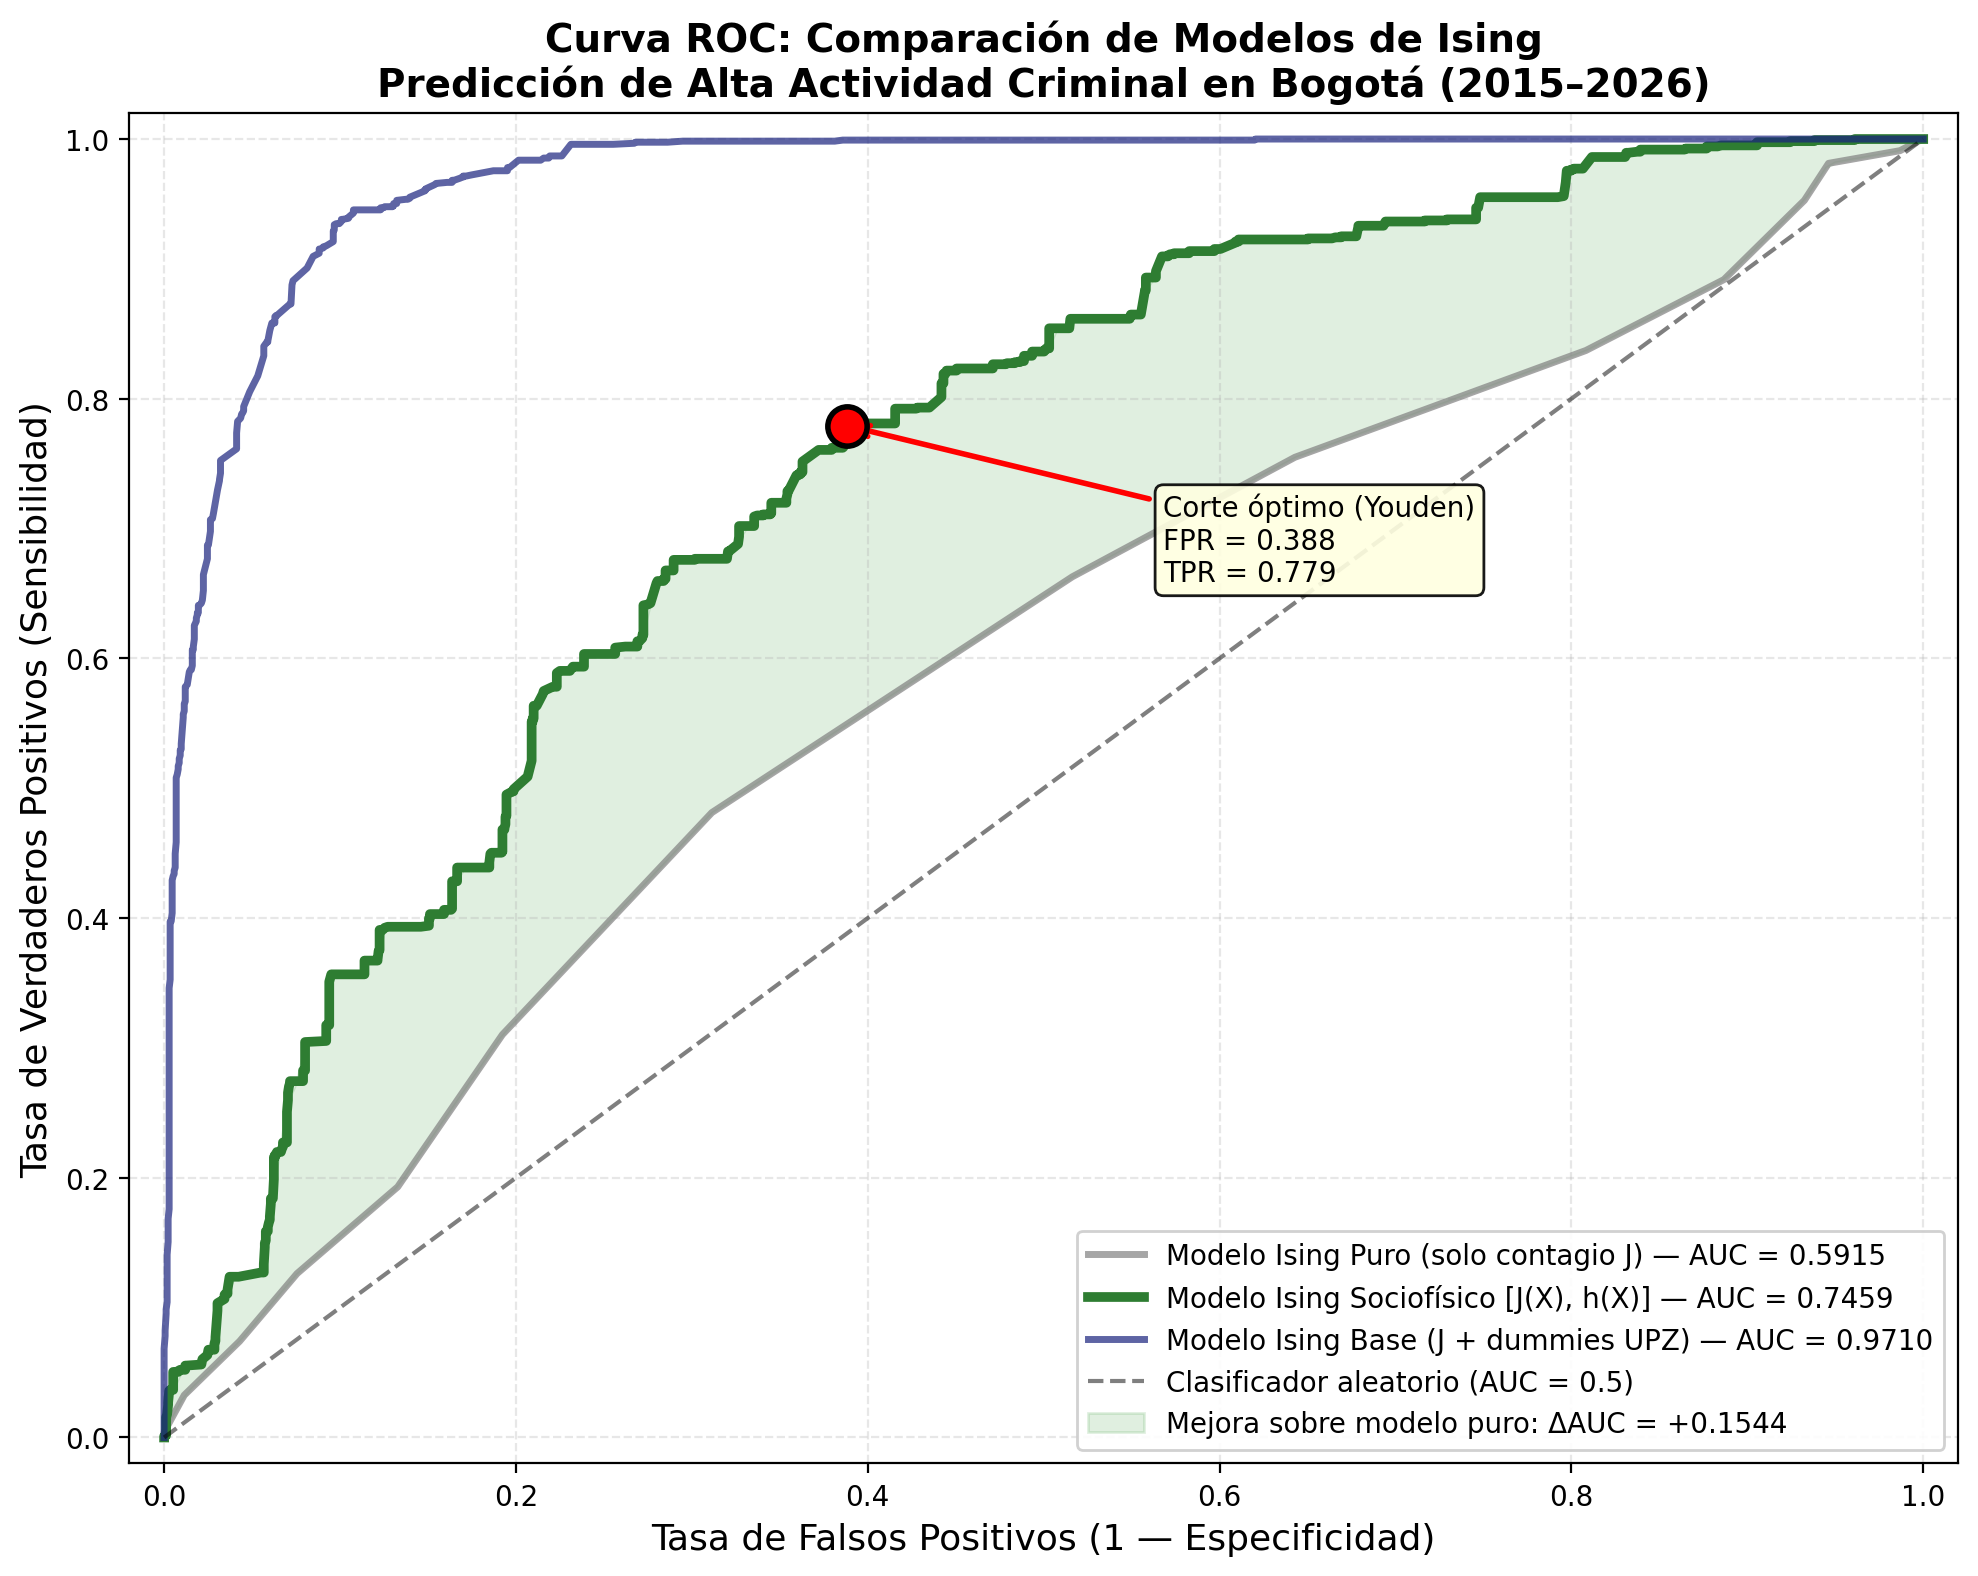
\includegraphics[width=0.78\textwidth]{graficas/fig1_curva_roc.png}
\end{center}
\vspace{-0.2cm}
\begin{center}
\small
Base: AUC = 0.971 \quad Sociofísico: AUC = 0.724 \quad Puro: AUC = 0.592

$\Delta\text{AUC} = +0.133$ (22.5\% de mejora). \textbf{Punto Youden:} FPR = 0.317, TPR = 0.681.
\end{center}
\end{frame}

\begin{frame}{Mapa de Campos Locales $h_i$}
\begin{center}
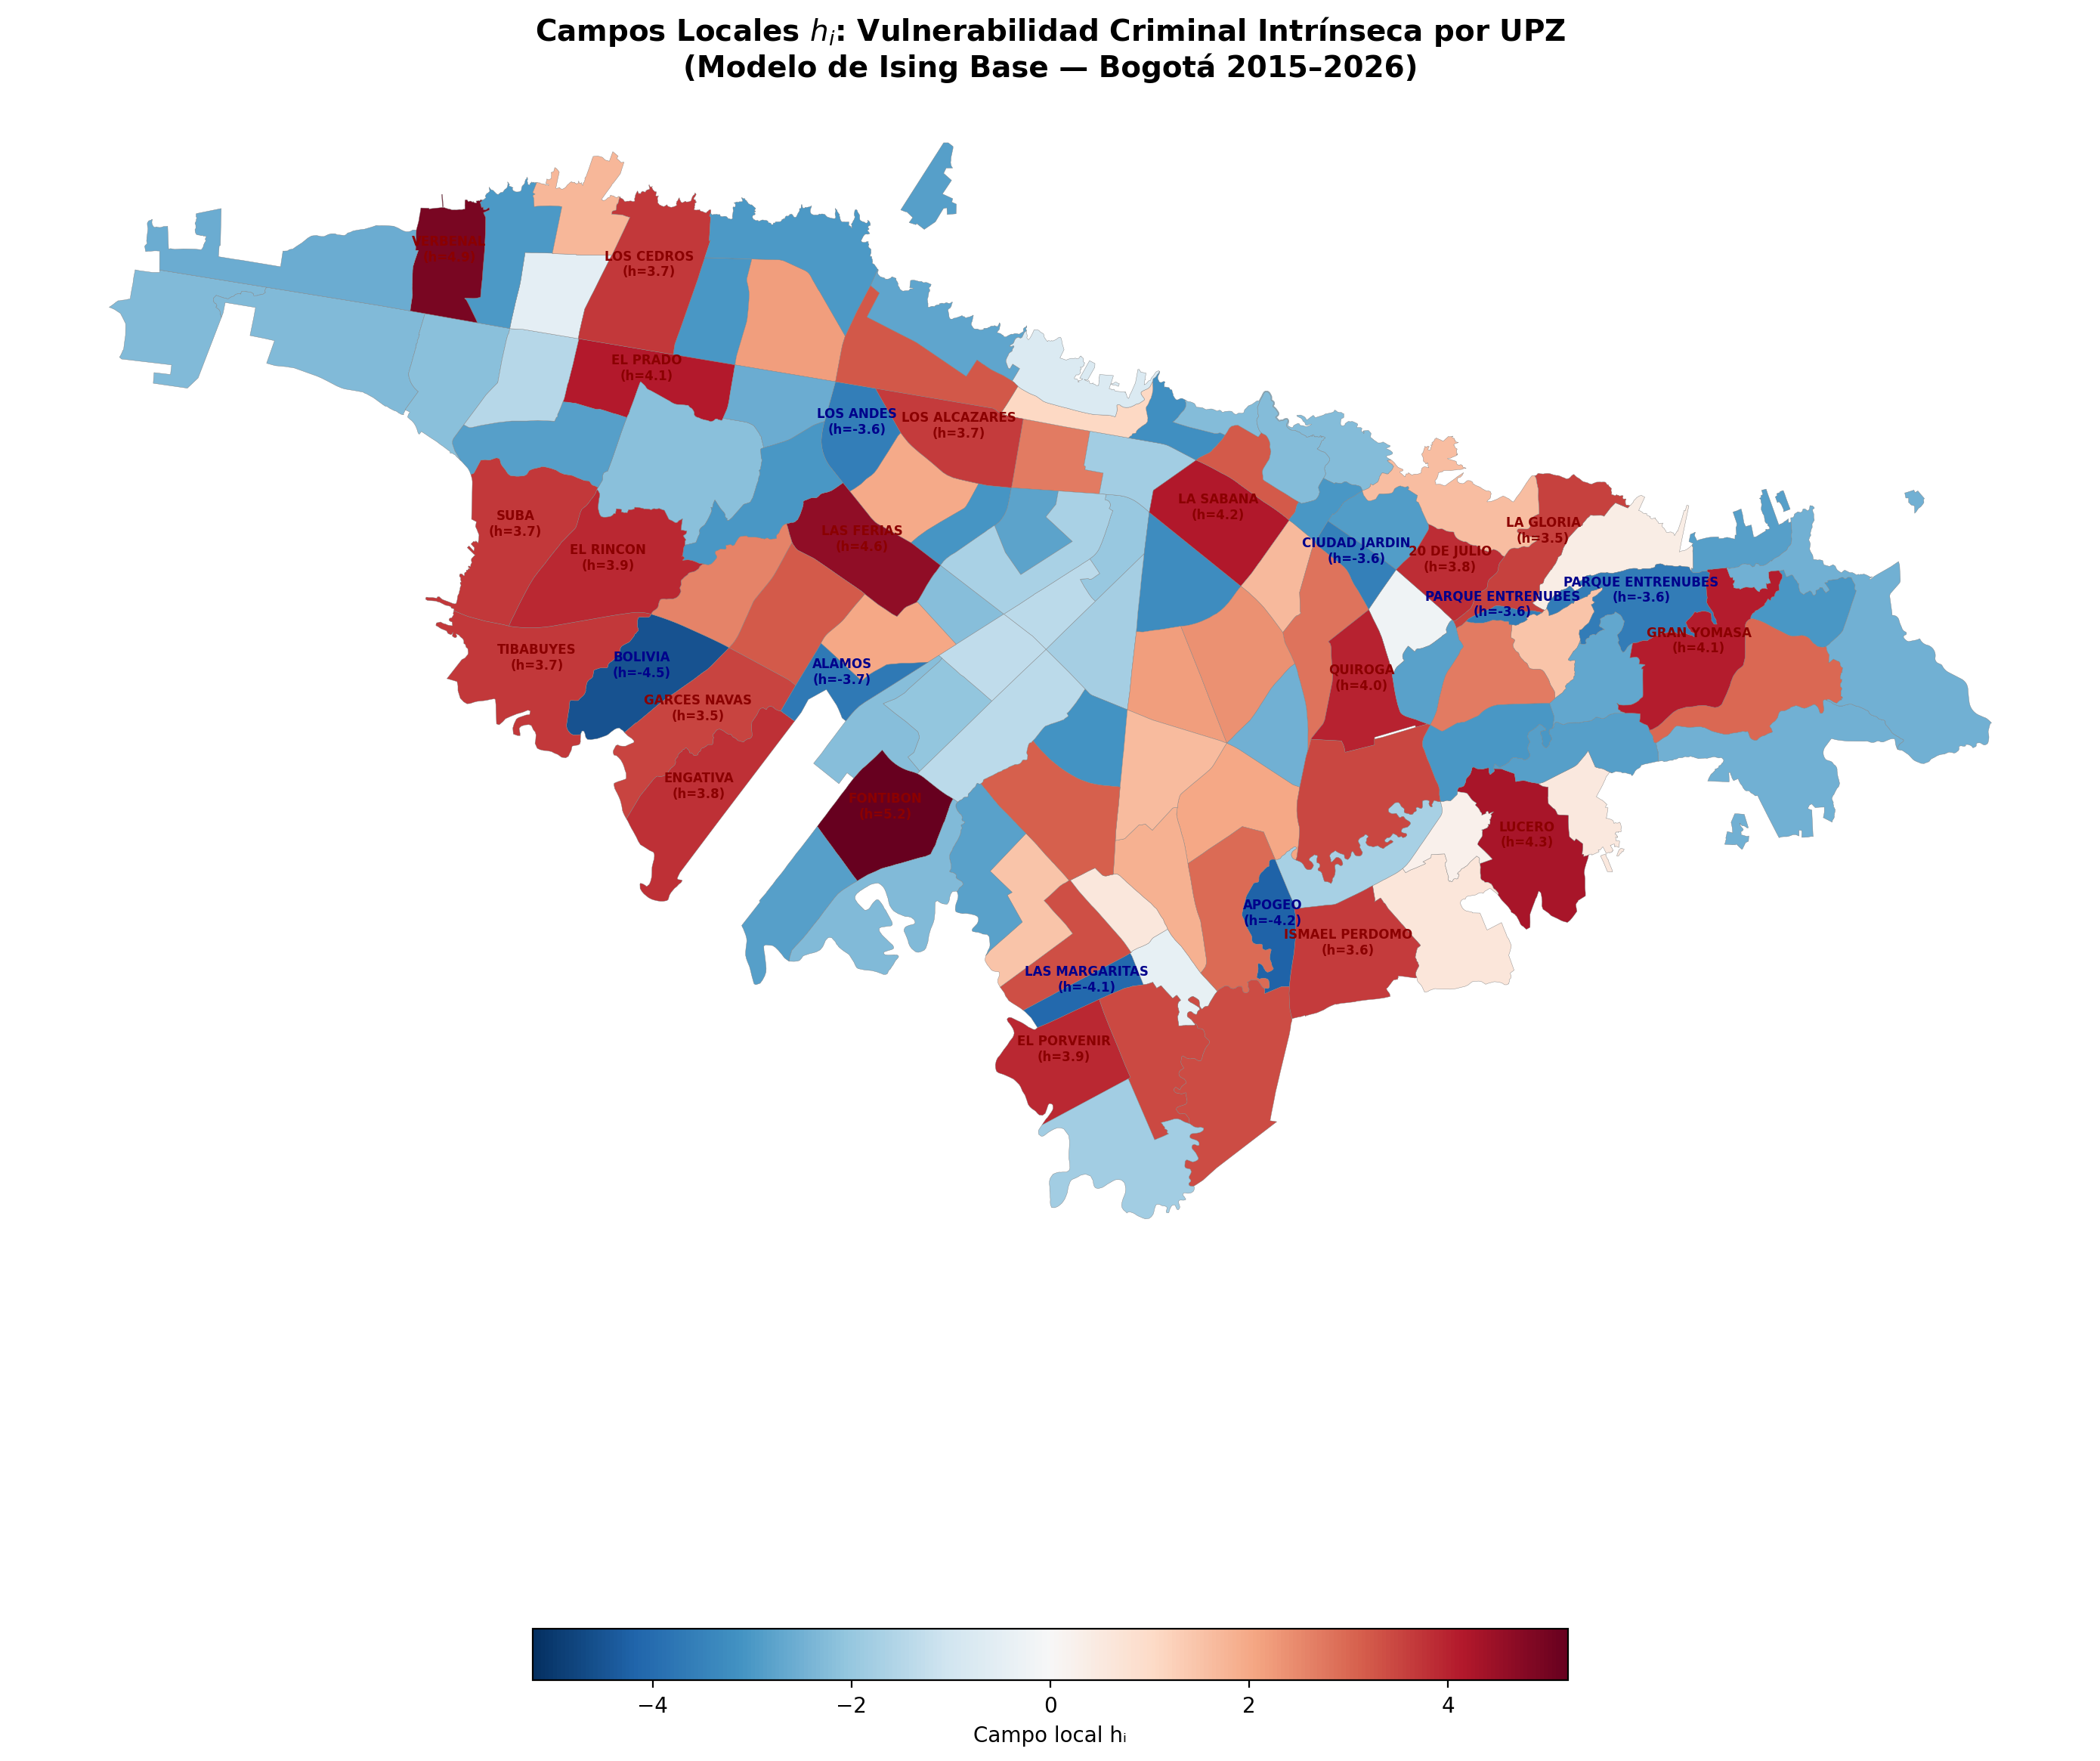
\includegraphics[width=0.68\textwidth]{graficas/fig2_mapa_campos_locales.png}
\end{center}
\vspace{-0.2cm}
\begin{center}
\small
Rojo: alta vulnerabilidad ($h_i > 0$). Azul: baja ($h_i < 0$).

Clusters en zona sur y noroccidental. Rango: $[-4.52, +5.21]$.
\end{center}
\end{frame}

\begin{frame}{Coeficientes del Modelo Sociofísico}

\begin{table}[h]
\centering
\small
\begin{tabular}{l r l}
\toprule
\textbf{Variable} & \textbf{Coef.} & \textbf{Efecto} \\
\midrule
\multicolumn{3}{c}{\textit{Efectos sobre el CONTAGIO ($J$)}} \\
\midrule
deserción\_promedio & $-0.085^{**}$ & BLOQUEA contagio \\
n\_cais & $+0.116^{***}$ & AMPLIFICA contagio \\
estrato\_medio & $+0.039^{*}$ & AMPLIFICA contagio \\
\midrule
\multicolumn{3}{c}{\textit{Efectos sobre el CAMPO LOCAL ($h$)}} \\
\midrule
deserción\_promedio & $+0.199^{***}$ & AUMENTA crimen \\
estrato\_medio & $-0.393^{***}$ & REDUCE crimen \\
n\_cais & $+0.088^{**}$ & AUMENTA crimen \\
\bottomrule
\end{tabular}
\end{table}

\vspace{0.15cm}
\begin{center}
La deserción crea ``islas'' de crimen. El estrato alto reduce crimen local pero amplifica contagio. Los CAIs son reactivos.
\end{center}
\end{frame}

\begin{frame}{Evolución del Poder Explicativo ($R^2$)}
\begin{center}
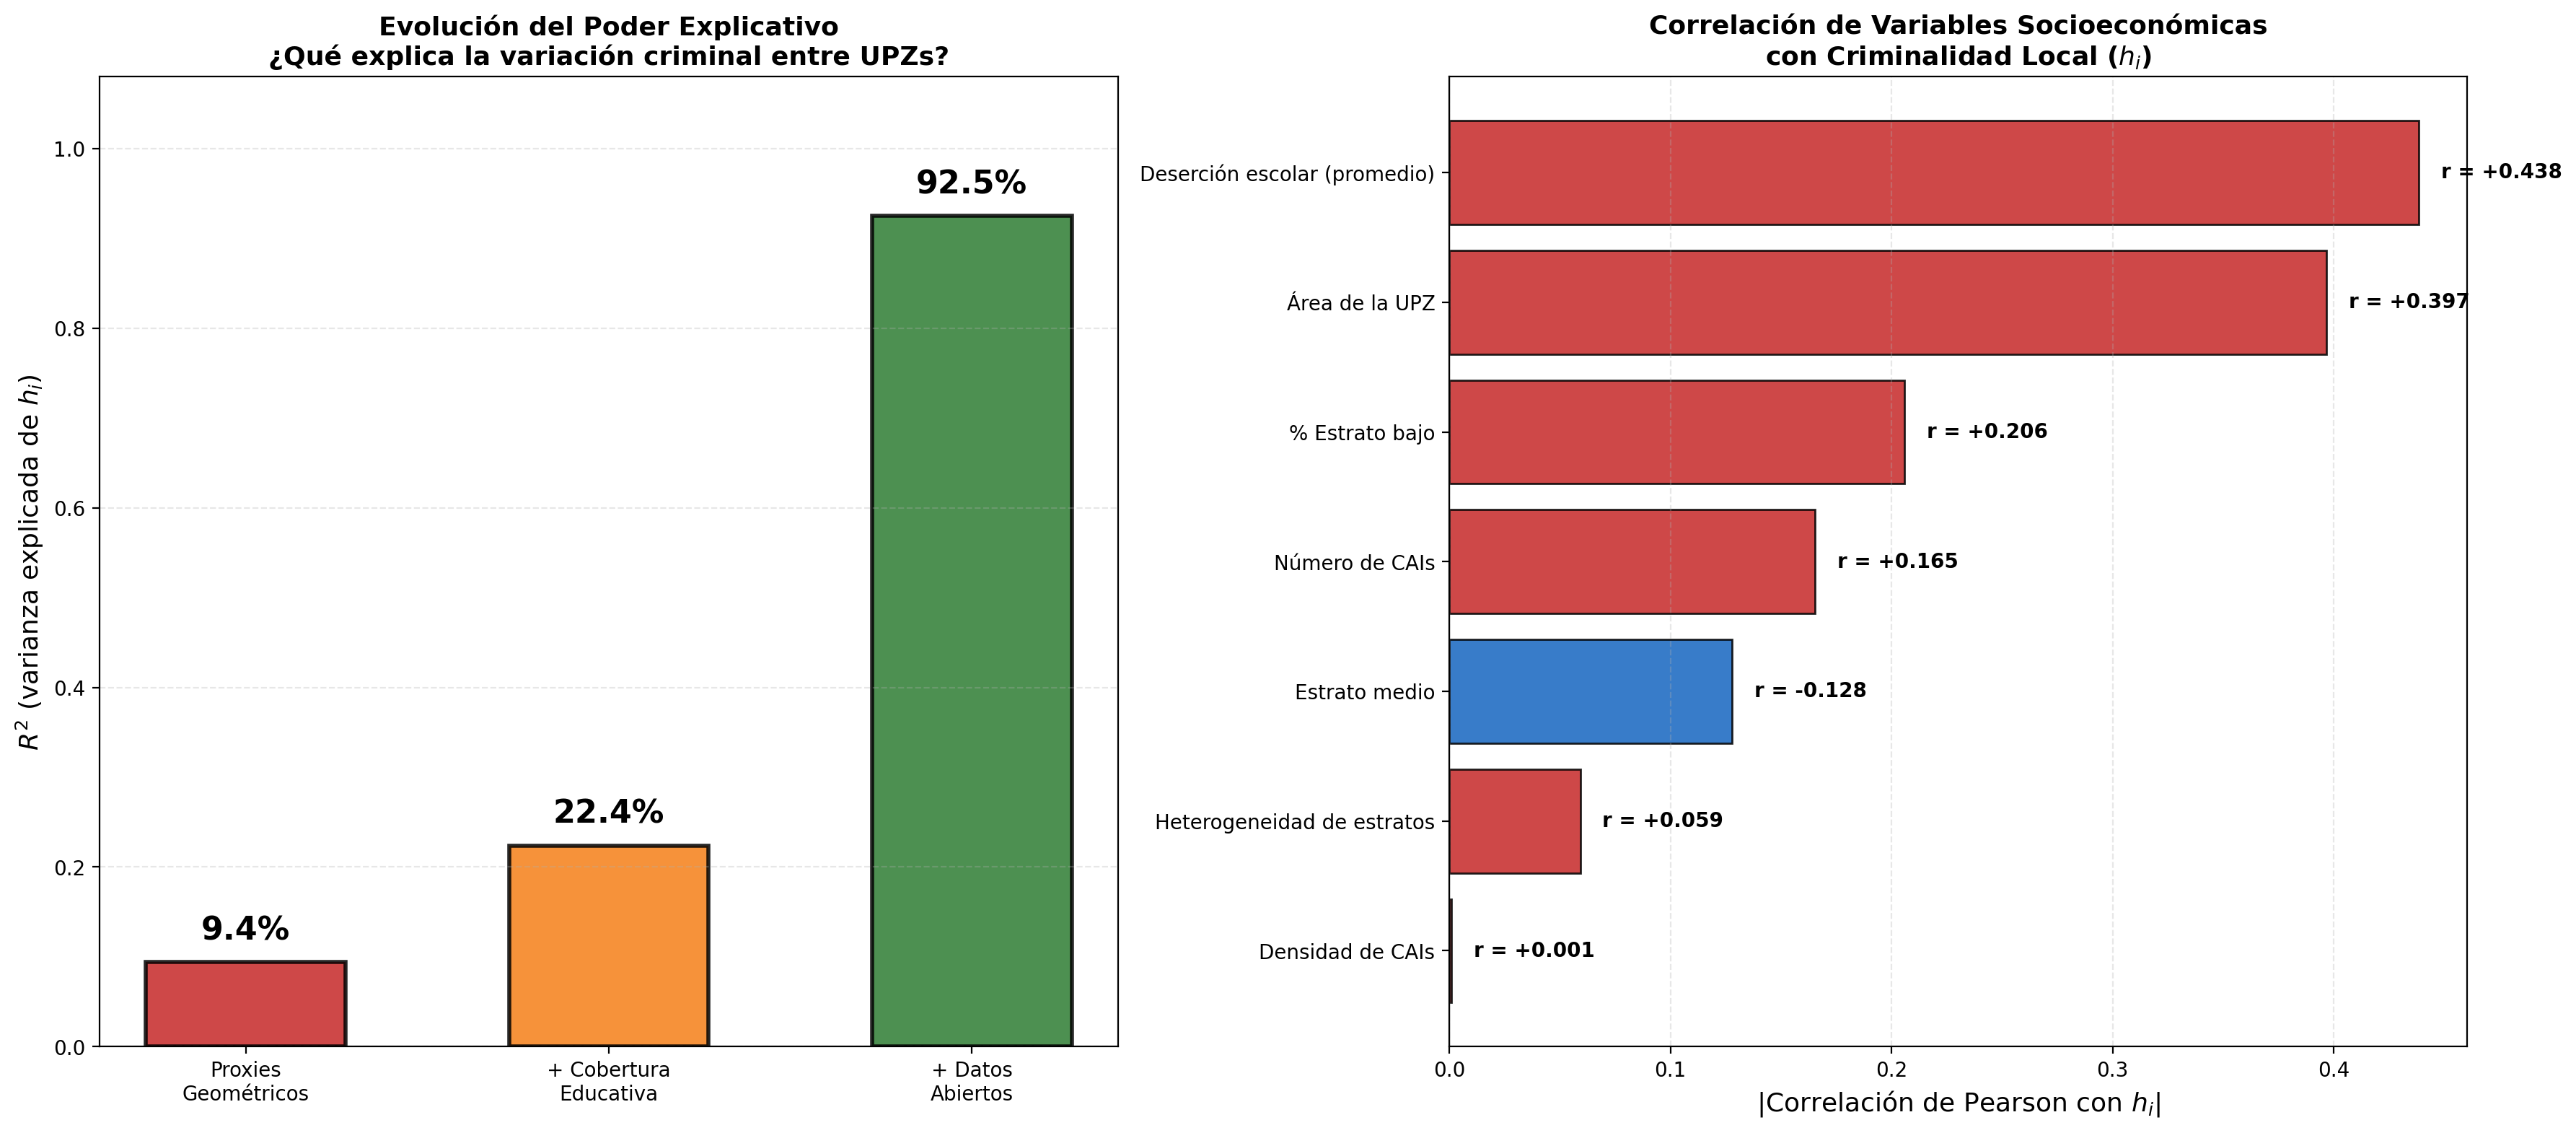
\includegraphics[width=0.95\textwidth]{graficas/fig4_evolucion_R2_correlaciones.png}
\end{center}
\vspace{-0.2cm}
\begin{center}
\small
Proxies geométricos: 9.4\% $\to$ Cobertura educativa: 22.4\% $\to$ \textbf{Datos abiertos: 92.5\%}

Mejora de 9.8$\times$. Variable más correlacionada: deserción\_min ($r = +0.539$, $p < 0.001$).
\end{center}
\end{frame}

\begin{frame}{Validación y Top 10 UPZs}

\begin{columns}[T]
\column{0.48\textwidth}
\textbf{Permutaciones (200):}
\begin{table}[h]
\centering
\scriptsize
\begin{tabular}{l c c c}
\toprule
 & \textbf{Obs.} & \textbf{Nulo} & \textbf{p} \\
\midrule
$C$ & 0.1210 & 0.1143 & \alert{$<0.001$} \\
$\chi$ & 2.78 & 28.96 & 1.000 \\
\bottomrule
\end{tabular}
\end{table}
\small
$C$ significativa: clusters reales.\\
$\chi$ no significativa: sin respuesta colectiva.

\column{0.52\textwidth}
\textbf{Mayor $h_i$:}
\begin{table}[h]
\centering
\scriptsize
\begin{tabular}{r l c c}
\toprule
 & \textbf{UPZ} & \textbf{$h_i$} & \textbf{Estr.} \\
\midrule
1 & FONTIBON & +5.21 & 2.8 \\
2 & VERBENAL & +4.93 & 3.0 \\
3 & LAS FERIAS & +4.61 & 2.6 \\
8 & QUIROGA & +3.99 & \textbf{1.0} \\
\bottomrule
\end{tabular}
\end{table}
\vspace{-0.2cm}
\scriptsize QUIROGA: estrato más bajo y alta deserción.
\end{columns}
\end{frame}

% ==================== SECCIÓN 5 ====================
\section{Discusión y Conclusiones}

\begin{frame}{Hallazgos Principales}

\begin{enumerate}
    \item \textbf{Deserción escolar:} Predictor \#1 ($r=+0.54$). Bloquea contagio ($-0.085$) pero aumenta crimen local ($+0.199$). Crea ``islas'' de crimen autónomo.
    
    \item \textbf{Estrato socioeconómico:} Efectos opuestos. Reduce crimen local ($-0.393$) pero amplifica contagio ($+0.039$). Zonas ricas son ``conductoras''.
    
    \item \textbf{CAIs:} Reactivos, no preventivos. Correlación positiva con crimen ($+0.088$) por endogeneidad en su ubicación.
    
    \item \textbf{Fase desordenada:} $T_{\text{eff}} = 1.29 > T_{\text{crit}} = 0.89$. Intervenciones puntuales tienen efectos impredecibles.
\end{enumerate}
\end{frame}

\begin{frame}{Implicaciones para Política Pública}

\begin{enumerate}
    \item \textbf{Intervención educativa:} Programas de retención escolar en UPZs con mayor $h_i$. Énfasis en hombres de grados 10-11.
    
    \item \textbf{Estrategia territorial:} UPZs grandes requieren estrategias de escala. Zonas de estrato alto necesitan control de contagio hacia vecinos.
    
    \item \textbf{Revisión de CAIs:} Evaluar efectividad real. Considerar redistribución hacia zonas con potencial preventivo.
    
    \item \textbf{Monitoreo de $T_{\text{eff}}$:} Alerta temprana para identificar ventanas de alta susceptibilidad.
    
    \item \textbf{Modelo predictivo:} AUC = 0.971 anticipa hotspots. $R^2 = 92.5\%$ identifica factores a intervenir.
\end{enumerate}
\end{frame}

\begin{frame}{Conclusiones}

\begin{enumerate}
    \item El modelo de Ising es una \textbf{herramienta viable y rigurosa} para modelar la dinámica criminal urbana.
    
    \item \textbf{Contagio validado:} $J = 0.4336$ ($p < 0.001$). El crimen se propaga entre UPZs vecinas.
    
    \item \textbf{Factores estructurales:} 92.5\% de $h_i$ explicado por variables observables. Deserción escolar es el predictor principal.
    
    \item \textbf{Marco interpretable:} El modelo descompone efectos sobre $J$ (contagio) y $h$ (campo local).
    
    \item \textbf{Herramienta de simulación:} Permite evaluar intervenciones antes de implementarlas.
    
    \item \textbf{Fase desordenada:} Intervenciones sostenidas son más efectivas que operativos puntuales.
\end{enumerate}
\end{frame}

\begin{frame}{Trabajo Futuro}

\vspace{0.2cm}

\begin{tabular}{p{0.28\textwidth} p{0.62\textwidth}}
\hline
\textbf{Línea} & \textbf{Descripción} \\
\hline
Datos adicionales & Alumbrado público, cámaras de seguridad, consumo de sustancias psicoactivas, violencia intrafamiliar \\
\hline
$J(t)$ dinámico & Ventanas móviles para capturar contagio variable en el tiempo \\
\hline
Validación externa & Evaluar predicciones con datos 2024--2025 no usados en el entrenamiento \\
\hline
Causalidad & Diseños cuasi-experimentales: diferencias en diferencias, regresión discontinua \\
\hline
Extensión geográfica & Aplicar la metodología a Medellín, Cali y otras ciudades colombianas \\
\hline
Movilidad & Incorporar datos de flujo de pasajeros en TransMilenio y SITP \\
\hline
\end{tabular}

\vspace{0.3cm}
\begin{center}
\small \textit{El modelo es extensible: nuevas covariables, otras ciudades, ventanas temporales.}
\end{center}
\end{frame}

% ==================== SECCIÓN FINAL ====================
\begin{frame}{Referencias}

\footnotesize
\begin{thebibliography}{99}
\bibitem{ising1925} E. Ising, \textit{Zeitschrift für Physik}, vol. 31, pp. 253--258, 1925.
\bibitem{castellano2009} C. Castellano et al., \textit{Reviews of Modern Physics}, vol. 81, pp. 591--646, 2009.
\bibitem{bogota_datos} Alcaldía Mayor de Bogotá, \texttt{datosabiertos.bogota.gov.co}, 2024.
\bibitem{anagnostopoulos2014}
K. N. Anagnostopoulos, \textit{Computational Physics, Vol I: A Practical Introduction to Computational Physics and Scientific Computing}, Lulu.com, 2014.
\bibitem{sklearn} F. Pedregosa et al., \textit{JMLR}, vol. 12, pp. 2825--2830, 2011.
\bibitem{geopandas} K. Jordahl et al., \texttt{geopandas.org}, 2024.
\bibitem{statsmodels} S. Seabold y J. Perktold, \textit{Proc. 9th Python in Science Conf.}, 2010.
\bibitem{numpy} C.R. Harris et al., \textit{Nature}, vol. 585, pp. 357--362, 2020.
\bibitem{pandas} W. McKinney, \textit{Proc. 9th Python in Science Conf.}, 2010.
\end{thebibliography}
\end{frame}

\begin{frame}
\centering
\Huge \textbf{¡Muchas gracias!}
\vspace{1cm}

\large \textbf{Comentarios y preguntas}

\vspace{1cm}
\normalsize
\textit{Modelo de Ising para Criminalidad en Bogotá}\\
\textit{Mecánica estadística · Universidad Distrital FJC · 2026}
\end{frame}

\end{document}